\documentclass{standalone}
\usepackage{tikz}
\usetikzlibrary{patterns, positioning}

\begin{document}
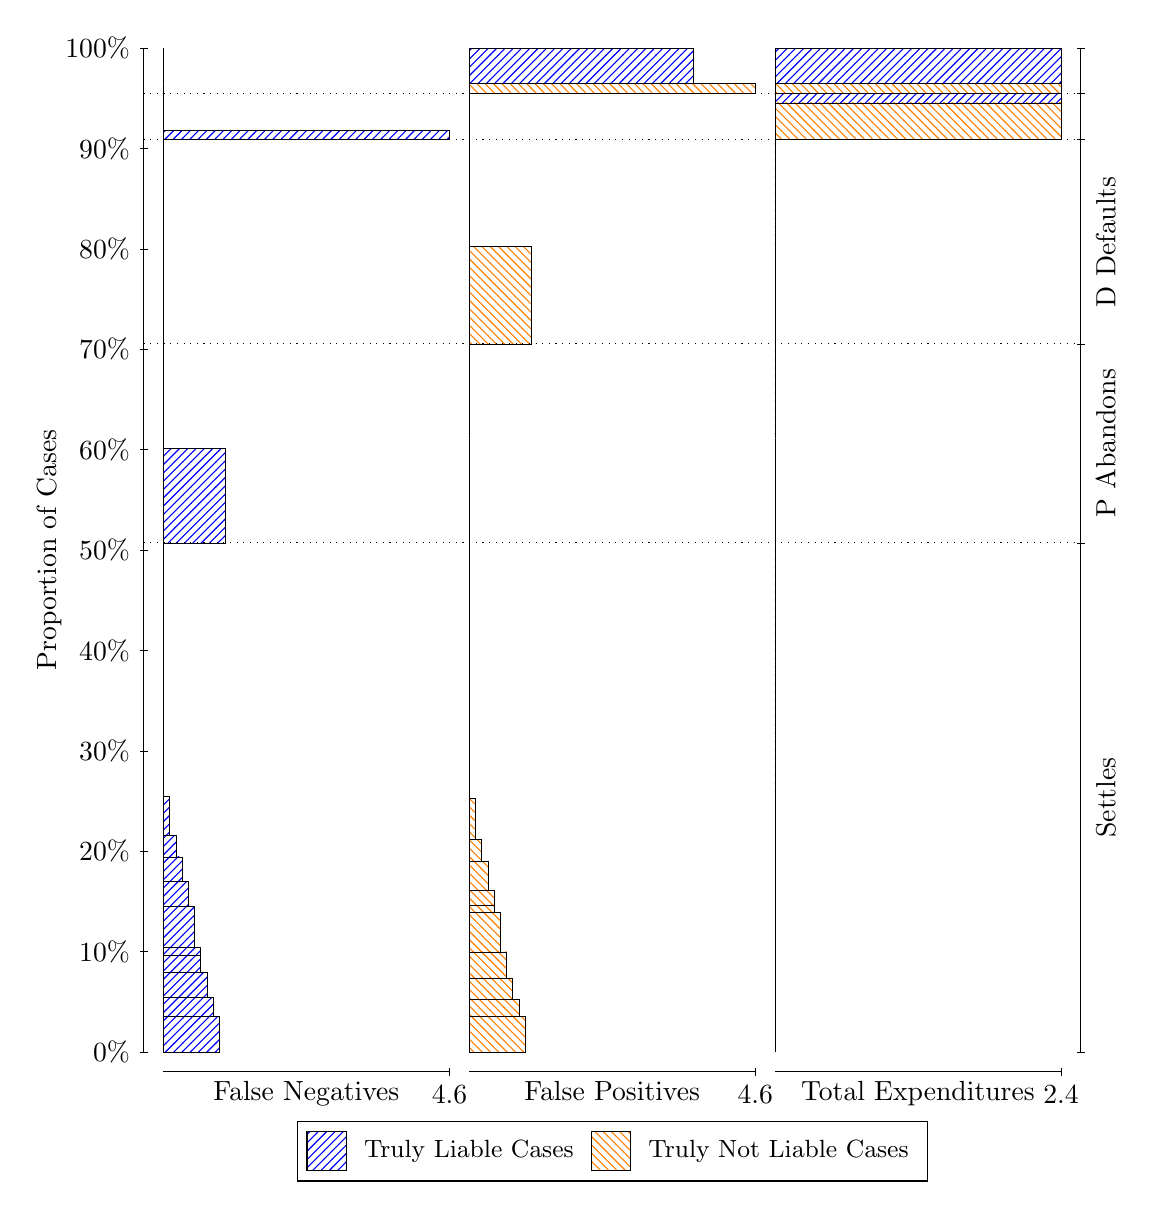
\begin{tikzpicture}
\draw[black, very thin] (1.5,1.75) -- (1.5,14.5);
\node[rotate=90, anchor=center] at (0.3, 8.125) {Proportion of Cases};
\draw[black, very thin] (1.45,1.75) -- (1.55,1.75);
\node[anchor=east] at (1.45, 1.75) {0\%};
\draw[black, very thin] (1.45,3.025) -- (1.55,3.025);
\node[anchor=east] at (1.45, 3.025) {10\%};
\draw[black, very thin] (1.45,4.3) -- (1.55,4.3);
\node[anchor=east] at (1.45, 4.3) {20\%};
\draw[black, very thin] (1.45,5.575) -- (1.55,5.575);
\node[anchor=east] at (1.45, 5.575) {30\%};
\draw[black, very thin] (1.45,6.85) -- (1.55,6.85);
\node[anchor=east] at (1.45, 6.85) {40\%};
\draw[black, very thin] (1.45,8.125) -- (1.55,8.125);
\node[anchor=east] at (1.45, 8.125) {50\%};
\draw[black, very thin] (1.45,9.4) -- (1.55,9.4);
\node[anchor=east] at (1.45, 9.4) {60\%};
\draw[black, very thin] (1.45,10.675) -- (1.55,10.675);
\node[anchor=east] at (1.45, 10.675) {70\%};
\draw[black, very thin] (1.45,11.95) -- (1.55,11.95);
\node[anchor=east] at (1.45, 11.95) {80\%};
\draw[black, very thin] (1.45,13.225) -- (1.55,13.225);
\node[anchor=east] at (1.45, 13.225) {90\%};
\draw[black, very thin] (1.45,14.5) -- (1.55,14.5);
\node[anchor=east] at (1.45, 14.5) {100\%};

\draw[black, very thin] (13.4,1.75) -- (13.4,14.5);
\draw[black, very thin] (13.35,1.75) -- (13.45,1.75);
\node[anchor=west] at (13.35, 1.75) {};
\draw[black, very thin] (13.35,8.2149) -- (13.45,8.2149);
\node[anchor=west] at (13.35, 8.2149) {};
\draw[black, very thin] (13.35,10.744) -- (13.45,10.744);
\node[anchor=west] at (13.35, 10.744) {};
\draw[black, very thin] (13.35,13.335) -- (13.45,13.335);
\node[anchor=west] at (13.35, 13.335) {};
\draw[black, very thin] (13.35,13.927) -- (13.45,13.927);
\node[anchor=west] at (13.35, 13.927) {};
\draw[black, very thin] (13.35,14.5) -- (13.45,14.5);
\node[anchor=west] at (13.35, 14.5) {};

\draw[black, very thin, pattern color=blue, pattern=north east lines] (1.75,1.75) rectangle (2.4609,2.202);
\draw[black, very thin, pattern color=blue, pattern=north east lines] (1.75,2.202) rectangle (2.3819,2.444);
\draw[black, very thin, pattern color=blue, pattern=north east lines] (1.75,2.444) rectangle (2.3029,2.7653);
\draw[black, very thin, pattern color=blue, pattern=north east lines] (1.75,2.7653) rectangle (2.2239,2.9789);
\draw[black, very thin, pattern color=blue, pattern=north east lines] (1.75,2.9789) rectangle (2.2239,3.0782);
\draw[black, very thin, pattern color=blue, pattern=north east lines] (1.75,3.0782) rectangle (2.1449,3.5941);
\draw[black, very thin, pattern color=blue, pattern=north east lines] (1.75,3.5941) rectangle (2.0659,3.9144);
\draw[black, very thin, pattern color=blue, pattern=north east lines] (1.75,3.9144) rectangle (1.987,4.2287);
\draw[black, very thin, pattern color=blue, pattern=north east lines] (1.75,4.2287) rectangle (1.908,4.5022);
\draw[black, very thin, pattern color=blue, pattern=north east lines] (1.75,4.5022) rectangle (1.829,4.999);
\draw[black, very thin, pattern color=orange, pattern=north west lines] (1.75,4.999) rectangle (1.75,8.2149);
\draw[black, very thin, pattern color=blue, pattern=north east lines] (1.75,8.2149) rectangle (2.5399,9.4171);
\draw[black, very thin, pattern color=orange, pattern=north west lines] (1.75,9.4171) rectangle (1.75,10.744);
\draw[black, very thin, pattern color=orange, pattern=north west lines] (1.75,10.744) rectangle (1.75,11.984);
\draw[black, very thin, pattern color=blue, pattern=north east lines] (1.75,11.984) rectangle (1.75,13.335);
\draw[black, very thin, pattern color=blue, pattern=north east lines] (1.75,13.335) rectangle (5.3833,13.458);
\draw[black, very thin, pattern color=orange, pattern=north west lines] (1.75,13.458) rectangle (1.75,13.927);
\draw[black, very thin, pattern color=orange, pattern=north west lines] (1.75,13.927) rectangle (1.75,14.05);
\draw[black, very thin, pattern color=blue, pattern=north east lines] (1.75,14.05) rectangle (1.75,14.5);
\draw[black, very thin, pattern color=orange, pattern=north west lines] (5.6333,1.75) rectangle (6.3442,2.1996);
\draw[black, very thin, pattern color=orange, pattern=north west lines] (5.6333,2.1996) rectangle (6.2652,2.4205);
\draw[black, very thin, pattern color=orange, pattern=north west lines] (5.6333,2.4205) rectangle (6.1862,2.6815);
\draw[black, very thin, pattern color=orange, pattern=north west lines] (5.6333,2.6815) rectangle (6.1072,3.0215);
\draw[black, very thin, pattern color=orange, pattern=north west lines] (5.6333,3.0215) rectangle (6.0283,3.5244);
\draw[black, very thin, pattern color=orange, pattern=north west lines] (5.6333,3.5244) rectangle (5.9493,3.6172);
\draw[black, very thin, pattern color=orange, pattern=north west lines] (5.6333,3.6172) rectangle (5.9493,3.8053);
\draw[black, very thin, pattern color=orange, pattern=north west lines] (5.6333,3.8053) rectangle (5.8703,4.1661);
\draw[black, very thin, pattern color=orange, pattern=north west lines] (5.6333,4.1661) rectangle (5.7913,4.4498);
\draw[black, very thin, pattern color=orange, pattern=north west lines] (5.6333,4.4498) rectangle (5.7123,4.9659);
\draw[black, very thin, pattern color=blue, pattern=north east lines] (5.6333,4.9659) rectangle (5.6333,8.2149);
\draw[black, very thin, pattern color=orange, pattern=north west lines] (5.6333,8.2149) rectangle (5.6333,9.5421);
\draw[black, very thin, pattern color=blue, pattern=north east lines] (5.6333,9.5421) rectangle (5.6333,10.744);
\draw[black, very thin, pattern color=orange, pattern=north west lines] (5.6333,10.744) rectangle (6.4232,11.984);
\draw[black, very thin, pattern color=blue, pattern=north east lines] (5.6333,11.984) rectangle (5.6333,13.335);
\draw[black, very thin, pattern color=orange, pattern=north west lines] (5.6333,13.335) rectangle (5.6333,13.804);
\draw[black, very thin, pattern color=blue, pattern=north east lines] (5.6333,13.804) rectangle (5.6333,13.927);
\draw[black, very thin, pattern color=orange, pattern=north west lines] (5.6333,13.927) rectangle (9.2667,14.05);
\draw[black, very thin, pattern color=blue, pattern=north east lines] (5.6333,14.05) rectangle (8.4768,14.5);
\draw[black, very thin, pattern color=orange, pattern=north west lines] (9.5167,1.75) rectangle (9.5167,4.9659);
\draw[black, very thin, pattern color=blue, pattern=north east lines] (9.5167,4.9659) rectangle (9.5167,8.2149);
\draw[black, very thin, pattern color=orange, pattern=north west lines] (9.5167,8.2149) rectangle (9.5167,9.5421);
\draw[black, very thin, pattern color=blue, pattern=north east lines] (9.5167,9.5421) rectangle (9.5167,10.744);
\draw[black, very thin, pattern color=orange, pattern=north west lines] (9.5167,10.744) rectangle (9.5167,11.984);
\draw[black, very thin, pattern color=blue, pattern=north east lines] (9.5167,11.984) rectangle (9.5167,13.335);
\draw[black, very thin, pattern color=orange, pattern=north west lines] (9.5167,13.335) rectangle (13.15,13.804);
\draw[black, very thin, pattern color=blue, pattern=north east lines] (9.5167,13.804) rectangle (13.15,13.927);
\draw[black, very thin, pattern color=orange, pattern=north west lines] (9.5167,13.927) rectangle (13.15,14.05);
\draw[black, very thin, pattern color=blue, pattern=north east lines] (9.5167,14.05) rectangle (13.15,14.5);
\draw[black, dotted] (1.5,8.2149) -- (13.4,8.2149);
\draw[black, dotted] (1.5,10.744) -- (13.4,10.744);
\draw[black, dotted] (1.5,13.335) -- (13.4,13.335);
\draw[black, dotted] (1.5,13.927) -- (13.4,13.927);
\draw[black, very thin] (1.75,1.5) -- (5.3833,1.5);
\node[anchor=north] at (3.5667, 1.5) {False Negatives};
\draw[black, very thin] (5.3833,1.45) -- (5.3833,1.55);
\node[anchor=north] at (5.3833, 1.45) {4.6};

\draw[black, very thin] (5.6333,1.5) -- (9.2667,1.5);
\node[anchor=north] at (7.45, 1.5) {False Positives};
\draw[black, very thin] (9.2667,1.45) -- (9.2667,1.55);
\node[anchor=north] at (9.2667, 1.45) {4.6};

\draw[black, very thin] (9.5167,1.5) -- (13.15,1.5);
\node[anchor=north] at (11.333, 1.5) {Total Expenditures};
\draw[black, very thin] (13.15,1.45) -- (13.15,1.55);
\node[anchor=north] at (13.15, 1.45) {2.4};

\node[black, centered, rotate=90] at (13.72, 4.9825) {Settles};
\node[black, centered, rotate=90] at (13.72, 9.4796) {P Abandons};
\node[black, centered, rotate=90] at (13.72, 12.04) {D Defaults};



\draw (7.449999999999999,1.5) node[draw=none] (baseCoordinate) {};
\begin{scope}[align=center]
        \matrix[scale=0.5, draw=black, below=0.5cm of baseCoordinate, nodes={draw}, column sep=0.1cm]{
            \node[rectangle, draw, minimum width=0.5cm, minimum height=0.5cm, pattern=north east lines, pattern color=blue] {}; &
            \node[draw=none, font=\small] (B) {Truly Liable Cases}; &
            \node[rectangle, draw, minimum width=0.5cm, minimum height=0.5cm, pattern=north west lines, pattern color=orange] {}; &
            \node[draw=none, font=\small] (B) {Truly Not Liable Cases}; \\
            };
\end{scope}

\end{tikzpicture}
\end{document}